\documentclass[hyperref, a4paper]{article}

\usepackage{geometry}
\usepackage{titling}
\usepackage{titlesec}
% No longer needed, since we will use enumitem package
% \usepackage{paralist}
\usepackage{enumitem}
\usepackage{footnote}
%\usepackage{enumerate}
\usepackage{amsmath, amssymb, amsthm}
\usepackage{mathtools}
\usepackage{bbm}
\usepackage{graphicx}
\usepackage[labelformat=simple]{subcaption}
\usepackage{physics}
\usepackage{tensor}
\usepackage{siunitx}
\usepackage[version=4]{mhchem}
\usepackage{tikz}
\usepackage{xcolor}
\usepackage{listings}
\usepackage{autobreak}
\usepackage[ruled, vlined, linesnumbered]{algorithm2e}
\usepackage{nameref,zref-xr}
\zxrsetup{toltxlabel}
\usepackage[sorting=none]{biblatex}
\addbibresource{tbg.bib}
\addbibresource{topo-band.bib}
\usepackage[colorlinks,unicode]{hyperref} % , linkcolor=black, anchorcolor=black, citecolor=black, urlcolor=black, filecolor=black
\usepackage[most]{tcolorbox}
\usepackage{prettyref}

% Page style
\geometry{left=3.18cm,right=3.18cm,top=2.54cm,bottom=2.54cm}
\titlespacing{\paragraph}{0pt}{1pt}{10pt}[20pt]
\setlength{\droptitle}{-5em}
%\preauthor{\vspace{-10pt}\begin{center}}
%\postauthor{\par\end{center}}

% More compact lists 
\setlist[itemize]{
    itemindent=17pt, 
    leftmargin=1pt,
    listparindent=\parindent,
    parsep=0pt,
}

% Math operators
\DeclareMathOperator{\polylog}{\mathrm{Li}}
\DeclareMathOperator{\arctanh}{\mathrm{arctanh}}
\DeclareMathOperator{\timeorder}{\mathcal{T}}
\DeclareMathOperator{\diag}{diag}
\DeclareMathOperator{\legpoly}{P}
\DeclareMathOperator{\primevalue}{P}
\DeclareMathOperator{\sgn}{sgn}
\DeclarePairedDelimiter\ceil{\lceil}{\rceil}
\DeclarePairedDelimiter\floor{\lfloor}{\rfloor}
\newcommand*{\ii}{\mathrm{i}}
\newcommand*{\ee}{\mathrm{e}}
\newcommand*{\const}{\mathrm{const}}
\newcommand*{\suchthat}{\quad \text{s.t.} \quad}
\newcommand*{\argmin}{\arg\min}
\newcommand*{\argmax}{\arg\max}
\newcommand*{\normalorder}[1]{: #1 :}
\newcommand*{\pair}[1]{\langle #1 \rangle}
\newcommand*{\fd}[1]{\mathcal{D} #1}
\DeclareMathOperator{\bigO}{\mathcal{O}}

% TikZ setting
\usetikzlibrary{arrows,shapes,positioning}
\usetikzlibrary{arrows.meta}
\usetikzlibrary{decorations.markings}
\tikzstyle arrowstyle=[scale=1]
\tikzstyle directed=[postaction={decorate,decoration={markings,
    mark=at position .5 with {\arrow[arrowstyle]{stealth}}}}]
\tikzstyle ray=[directed, thick]
\tikzstyle dot=[anchor=base,fill,circle,inner sep=1pt]

% Algorithm setting
% Julia-style code
\SetKwIF{If}{ElseIf}{Else}{if}{}{elseif}{else}{end}
\SetKwFor{For}{for}{}{end}
\SetKwFor{While}{while}{}{end}
\SetKwProg{Function}{function}{}{end}
\SetArgSty{textnormal}

\newcommand*{\concept}[1]{{\textbf{#1}}}

% Embedded codes
\lstset{basicstyle=\ttfamily,
  showstringspaces=false,
  commentstyle=\color{gray},
  keywordstyle=\color{blue}
}

% Reference formatting
\renewcommand\thesubfigure{(\alph{subfigure})}
\newrefformat{fig}{Fig.~\ref{#1}}
\newrefformat{subfig}{Fig.~\ref{#1}(\subref{#1})}

% Color boxes
\tcbuselibrary{skins, breakable, theorems}
\newtcbtheorem[number within=section]{warning}{Warning}%
  {colback=orange!5,colframe=orange!65,fonttitle=\bfseries, breakable}{warn}
\newtcbtheorem[number within=section]{note}{Note}%
  {colback=green!5,colframe=green!65,fonttitle=\bfseries, breakable}{note}
\newtcbtheorem[number within=section]{info}{Info}%
  {colback=blue!5,colframe=blue!65,fonttitle=\bfseries, breakable}{info}

\newenvironment{shelldisplay}{\begin{lstlisting}}{\end{lstlisting}}

\title{Twisted bilayer graphene}
\author{Jinyuan Wu}

\begin{document}
    
\maketitle

\section{Introduction}

The mechanisms of \ce{Fe}- and \ce{Cu}-based high-$T_{\text{c}}$ superconductivity 
are still open problems in condensed matter physics.
Since in both types of systems, 
there are stacked conducting planes, 
a natural idea is to build monolayer materials to reproduce the behaviors observed in 
unconventional superconductivity.

It is well known that the band structure in graphene 
is highly sensitive to stacking,
and stacked bilayer graphene generally has 
a twisted angle $\theta$ between two layers of graphene,
forming Moire patterns.
An early DFT results reveal that when 
$\theta$ is around \SI{1.5}{\degree},
a drastic band flattening occurs,
which has the potential to induce correlated electronic phases 
and is experimentally verified in \cite{li_observation_2010}.
Semi-analytic analysis has revealed that 
at so-called magical angles (the smallest being $\theta \approx \SI{1.1}{\degree}$), 
the Fermi velocity drops to zero
\cite{bistritzer_moire_2011}.
\cite{cao_correlated_2018,cao_unconventional_2018} 
improves the control of $\theta$ and 
experimentally observe correlated insulating states when $\theta$ is around the first magical angle 
and the unconventional superconductivity when the system is slightly doped away from the insulator phase
with a phase diagram similar to that of cuprates.

This report reviews relevant theoretical and experimental progress 
in understanding twisted bilayer graphene.
\prettyref{sec:lattice} discusses related

\section{The lattice structure}\label{sec:lattice}

\begin{figure}
    \centering
    \begin{subfigure}{0.2\textwidth}
        \centering
        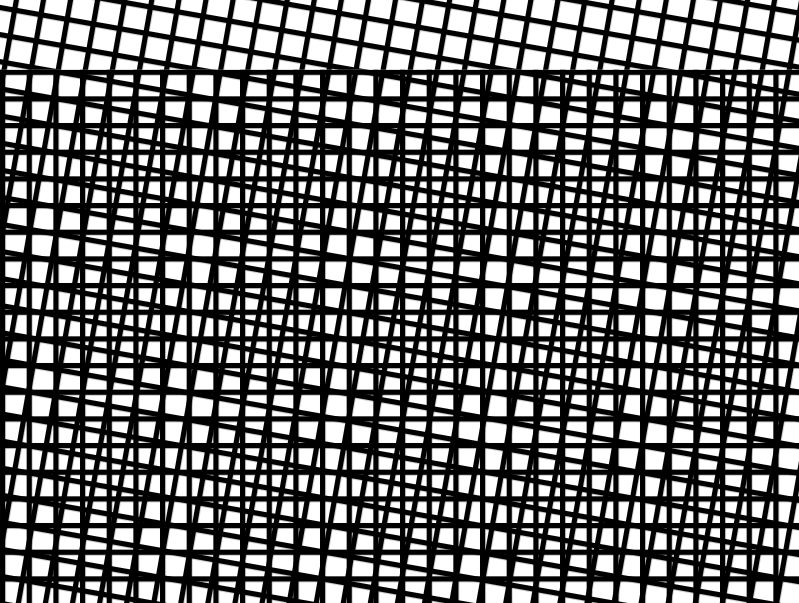
\includegraphics[width=\textwidth]{structure/moire-square.png}
        \subcaption{}
        \label{fig:square-moire}
    \end{subfigure}    
    \begin{subfigure}{0.3\textwidth}
        \centering
        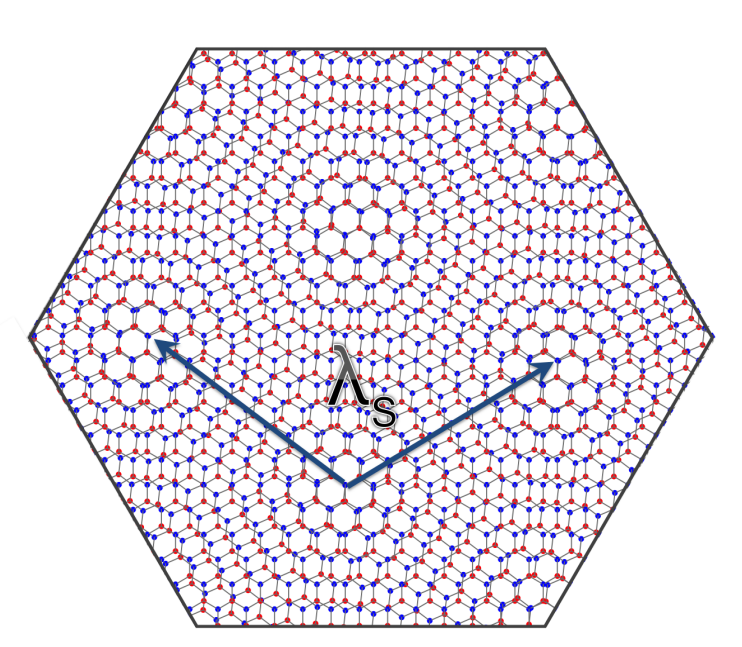
\includegraphics[width=\textwidth]{structure/moire-graphene.PNG}
        \subcaption{}
        \label{fig:hexagonal-moire}
    \end{subfigure}
    \begin{subfigure}{0.3\textwidth}
        \centering
        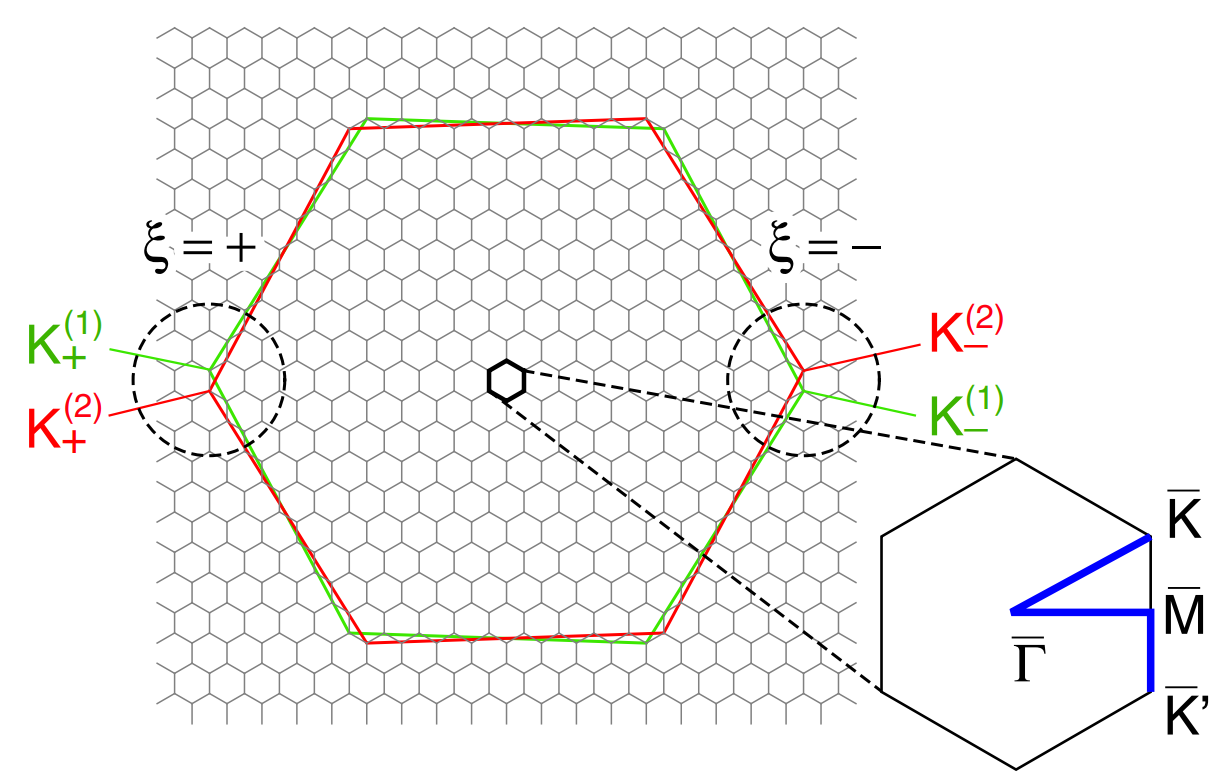
\includegraphics[width=\textwidth]{structure/moire-k-graphene.PNG}
        \subcaption{}
        \label{fig:1bz-1}
    \end{subfigure}
    \caption{Moire patterns in condensed matter physics.
    (a) Moire pattern of twisted bilayer square lattice. 
    Picture taken from \href{https://en.wikipedia.org/wiki/Moir\%C3\%A9\_pattern\#/media/File:Moir\%C3\%A9\_grid.svg}{Wikipedia}.
    (b) Twisted bilayer graphene in real space. Image from Fig. 1(b) in \cite{padhi_doped_2018}.
    The length $\lambda_\text{s}$ is the lattice constant of the hexagonal supercell.
    Note that $\lambda_{\text{s}}$ is the distance between the centers of two nearest supercells,
    but \emph{not} the length of each side of the supercell:
    it is $\sqrt{3}$ times of the length of each side of the supercell.
    (c) The first Brillouin zone of the two layers in (b) (red and green),
    and the first Brillouin zone (the black hexagon at the center) of the whole system.
    Image from Fig. 1(c) in \cite{koshino_band_2019}.
    The labels $\xi = \pm 1$ are valley labels 
    (marking the two nonequivalent Dirac cones in the first Brillouin zone of graphene),
    and K$+$ and K$-$ may alternatively be referred to as K abd K',
    and the labels (1) and (2) are layer labels.
    }
\end{figure}

Let us begin with the easier case of twisted square lattices.
Consider \prettyref{fig:square-moire}, 
and suppose $\vb*{a}_1$ is the primitive lattice vector in the $x$ direction,
and $\vb*{a}_2$ is the primitive lattice vector in the $y$ direction.
We choose the origin to be a point 
that is a lattice point of both layers.
In \prettyref{fig:square-moire} we can observe supercell-like patterns,
and the origin point may be seen as the center of one supercell.
Any other point that is a lattice point of both layers, then,
has to be the center of another supercell.

Now suppose we are to calculate the distance between two nearest supercells 
on the $x$ direction in \prettyref{fig:square-moire}.
Assume the two layers of lattices are commensurate.
Suppose $n \vb*{a}_2$ connects the two unit cells.
From the condition that the center of a supercell is 
a lattice point of both lattices, 
we have
\begin{equation}
    n \vb*{a}_2 = m \vb{R} \vb*{a}_2 + \vb*{a}_1.
    \label{eq:supercell-eq-origin}
\end{equation}
Here $\vb{R}$ is the rotation matrix;
the difference between $n \vb*{a}_2$ and $m \vb{R} \vb*{a}_2$ 
should be roughly in the $x$ direction, 
and it should be minimal, so we take it to be $\vb*{a}_1$.%
\footnote{
    To be exact, it may not be $\vb*{a}_1$, but, say, $10 \vb*{a}_1 + \vb*{a}_2$,
    and if the latter value is the case,
    the supercell built according to \eqref{eq:supercell-eq-origin} is just an approximate supercell; 
    but usually this approximation is already good enough -- 
    see the discussion on incommensurability below.
}
Since the rotation angle is not very large,
if $n \vb*{a}$ is between two nearest supercells, 
we have $m \approx n$
(because in this case the lengths of $n \vb*{a}_2$ and $m R \vb*{a}_2$ should be approximately the same),
and therefore we get 
\begin{equation}
    \text{lattice constant of supercell} = n a = a / \tan \theta \approx \frac{na}{\theta}.
    \label{eq:supercell-sq}
\end{equation}

Now we move to the twisted bilayer construction of graphene (\prettyref{fig:hexagonal-moire}).
Following the logic of \eqref{eq:supercell-eq-origin},
we have 
\begin{equation}
    \text{lattice constant of supercell} \approx \frac{na}{\theta}
\end{equation}
again. Note that here the lattice constants of both the honeycomb structure of each layer and the supercell 
are \emph{not} the bond length:
it is $\sqrt{3}$ times of the bond length.
Suppose we draw a vector $\vb*{\lambda}_{\text{s}}$ 
from the center of one unit cell to the unit cell directly above it,
and then rotate it with the angle $\theta$.
By the definition of ``center of one unit cell'' above,
we have $\Delta \vb*{\lambda}_{\text{s}}$ equal to a lattice vector,
but $\Delta \vb*{\lambda}_{\text{s}}$ is roughly in the $x$ direction 
and is not parallel to any bond in \prettyref{fig:hexagonal-moire}:
the length of the shortest lattice vector in the $x$ direction is 
the lattice constant of the honeycomb structure.%
\footnote{
    Recall that the graphene structure is a non-Bravais lattice.
    $\sqrt{3}$ times the bond length is exactly the length of a primitive lattice vector 
    if we reconsider the graphene structure as a Bravais lattice 
    with a two-atom basis.
}

With the supercell established in \prettyref{fig:hexagonal-moire},
we now consider the corresponding phenomenon in the reciprocal space
(\prettyref{fig:1bz-1}).
The uncertainty principle tells us that an increased unit cell in the real space 
means a shrunk first Brillouin zone.
Under the commensurability condition imposed above,
we indeed have a first Brillouin zone corresponding to the supercell
(which is called the ``mini Brillouin zone'' in \cite{cao_correlated_2018,cao_unconventional_2018}),
which should be the ``greatest common divisor'' of both layers.
The ``common divisor'' part means the two first Brillouin zones of the two layers 
are hexagon on the lattice points of the tessellation 
of the first Brillouin zone corresponding to the supercell,
and the ``greatest'' part means the first Brillouin zone corresponding to the supercell
should be as large as possible.
Considering the orientation of the supercell,
what we find is \prettyref{fig:1bz-1}.

If we twist two ideal lattices with an arbitrary angle and stack them,
that the two lattices are commensurate is not guaranteed,
so the resulting material is not periodic,
which may block electric currents.
What makes this structure different from non-periodic systems like quasicrystals or amorphous is 
even when the two layers of lattices are not commensurate,
we can still see approximate supercells,
though with a varying lattice constant.
However, when $\theta$ is close to zero,
values of commensurate $\theta$ are highly dense,
so with any $\theta$ the system is approximately periodic \cite{yao_quasicrystalline_2018}.
In practice, even prototypical crystals have spatially varying distortion of the lattice structure,
and the incommensurability of the two layers seems to have nothing different from that:
it can be well modeled by two commensurate layers plus small distortion.
The quasi-periodic supercells may further be regularized into a truly periodic structure by lattice relaxation.
Therefore, the procedure used to derive \eqref{eq:supercell-sq} is used
whenever $\theta$ is close to zero enough,
and the commensurate picture can always be used.%
\footnote{
    The incommensurability case can still be handled fully analytically \cite{catarina_twisted_2019},  
    but this is beyond the coverage of this report.
}

\section{Band theory and engineering of flat bands}

\begin{figure}
    \centering
    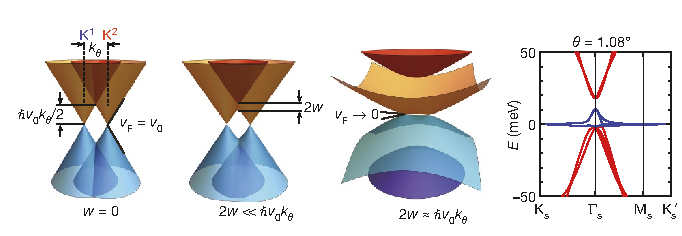
\includegraphics[width=0.8\textwidth]{plot/yuan-cao-band.pdf}
    \caption{Flat band at the magical angle. Figure from \cite{cao_correlated_2018}.
    The symbol $w$ gives inter-band hybridization.}
    \label{fig:flat-band-generation}
\end{figure}

A hand-waving argument about what happens after Brillouin zone folding happens according to \prettyref{fig:1bz-1}
is given in \cite{cao_correlated_2018},
illustrated in \prettyref{fig:flat-band-generation}.
In \prettyref{fig:1bz-1}, it can be seen that 
the equivalent band valleys of the upper layer and the lower layer 
(denoted by $\mathrm{K}^{(1)}_+$ and $\mathrm{K}^{(2)}_+$)
are folded to the K point and K' point of the mini Brillouin zone,
and the two Dirac cone cross each other.
When inter-layer hopping is present,
the crossings tend to be avoided,
and the two intersecting Dirac cones split into four bands,
the highest and the lowest being blunt cones.
Since time reversal symmetry and spatial inversion symmetry are always present,
the middle two bands are always connected by two Dirac points.
When hybridization is strong, the gap between the highest and the lowest bands 
and the two bands near the Fermi level is increased,
and the two Dirac points are always present,
so the two bands are flattened around the Dirac points.
The result band structure has almost zero Fermi velocity near the Dirac points 
$\mathrm{K}_{\text{s}}$  and $\mathrm{K}'_{\text{s}}$ in the mini Brillouin zone.
Note that here we have 8 flat bands:
two Dirac cones from two layers are involved in band flattening,
and in each Dirac cone there are two spins,
and there are two two nonequivalent valleys 
(so there are two pairs of Dirac cones, 
each pair of which undergo band flattening).

Working out an effective band description of the twisted bilayer graphene system 
is important in understanding its b

\section{Correlation electronic states}



\section{Conclusion}

\printbibliography

\end{document}